\documentclass{classrep}
\usepackage[utf8]{inputenc}
\usepackage{color}
\usepackage{graphicx}
\usepackage[section]{placeins}

\DeclareUnicodeCharacter{00A0}{~}

\studycycle{Informatyka, studia dzienne, inż I st.}
\coursesemester{IV}

\coursename{Sztuczna inteligencja i systemy ekspertowe}
\courseyear{2023/2024}

\courseteacher{Dr. Krzysztof Lichy}
\coursegroup{poniedziałek, 12:15}

\author{
    \studentinfo{Mateusz Giełczyński}{247662} \and
    \studentinfo{Jakub Kubiś}{247712}
}

\title{Zadanie 1: Piętnastka}

\begin{document}
    \maketitle





    \section{Cel}
    {
        Celem zadania było napisanie programu znajdującego rozwiązanie układanki logicznej zwanej "Pietnastką" oraz zbadanie zasad działania
        algorytmów przeszukujących grafy.
    }\label{sec:cel}

    \section{Wprowadzenie}
    {

     Piętnastka to układanka logiczna składająca się z kwadratowej
        planszy podzielonej na 16 kwadratów. Zawierających cyfry od 1 do 15 oraz jednym miejscem które zawsze pozostaje puste
        co pozwala na przesuwanie sąsiednich kafelków, celem piętnastki jest uporządkowanie kafelków tak aby uzyskać układ liczbowy
        gdzie liczby ułożone są w porządku rosnącym, a ostatnie pole pozostaje puste.




        Piętnastkę można zinterpretować jako graf, gdzie danym węzłem jest stan planszy. Natomiast krawędzie łączące węzły
    reprezentują możliwe ruchy pomiędzy stanami. Korzeniem w takim grafie będzie początkowy nierozwiązany stan układanki.

    Inepretacja piętnastki jako grafu pozwala nam stosować metody przeszukiwania grafów do znajdywania rozwiązań układnaki.
    Zaimplementowane przez nas metody to:
        \begin{itemize}
            \item BFS (breadth-first search) - przeszukiwanie wszerz.

            Metoda polega na przeszukaniu wszystkich węzłów na jednej głębokości przed zejściem na niższy poziom.
            \item DFS (depth-first search) - przeszukiwanie wgłąb.

            Metoda polega na przeszukiwaniu w głąb, oznacza to że zanim zbada kolejną krawedź pierwszego węzła
            dopiero gdy zbada wszystkie krawędzie kolejnego węzła.
            \item A* (A-star).

            Metoda polega na wybieraniu najbardziej obiecujacego węzła na podstawie heurystyki.
            \begin{itemize}
                \item Heurystyka Hamminga

                Heurystyka polega na zliczeniu ilości kafelków które nie znajdują się na odpowiednim miejscu.
                \item Heurystyka Manhattana

                Heurystyka polega na zliczeniu sumy ruchów, które potrzebuje każdy z kafelków, żeby znależć się na odpowiednim miejscu.
            \end{itemize}
        \end{itemize}
        \begin{figure}[!ht]
            \centering
            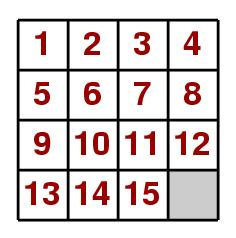
\includegraphics[width=0.6\textwidth,keepaspectratio]
            {15}
            \caption{Rozwiązana piętnastka}
            \label{fig:Rozwiązana piętnastka}
        \end{figure}
    }\label{sec:wprowadzenie}

    \section{Opis implementacji}
    {
        Program został stworzony w języku Python 3.

        Klasa Board odpowiada za przechowywanie stanu planszy, związanych z nią informacji oraz przemieszczanie elementów planszy.

    Klasa Solver oraz klasy po niej dziedziczące zawierają logikę odpowiedzalną za rozwiązanie układanki daną metodyką.

    Klasa Logger odpowiada za zbieraniu dodatkowych informacji, może być połaczona z klasami rozwiązującymi korzystając ze wzorca projektowego obserwatora zaimplemetowanego poprzez klasy ObserverMixin oraz ObservableMixin.

        \begin{figure}[!htb]
            \centering
            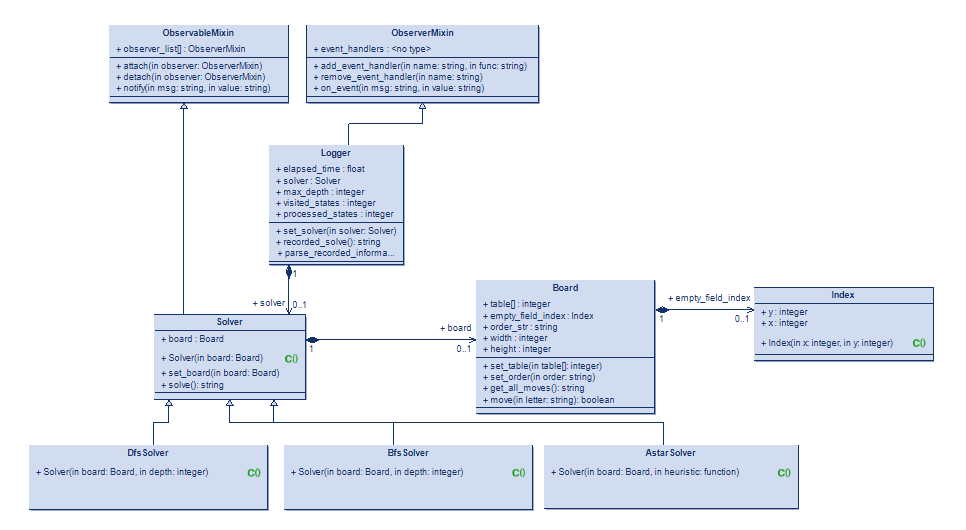
\includegraphics[width=\textwidth,height=\textheight,keepaspectratio]{diagram}
            \caption{Diagram UML}
            \label{fig:Diagram UML}
        \end{figure}
     \label{sec:opis-implementacji}}


    \section{Materiały i metody}
    {
        Do przeprowadzenia eksperymentów użyto narzędzi udostępnionych na platformie WIKAMP,
        zostały wykorzystane przy:
        \begin{itemize}
            \item Generowaniu stanów układanek do rozwiązania
            \item Uruchamianiu wykonanego programu dla wygenerowanych układanek
            \item Weryfikacji poprawności rozwiązań
            \item Podsumowaniu wyników
        \end{itemize}
        Badania zostały przeprowadzone dla wszystkich metod oraz wszystkich możliwych stanów dla
        głębokości od 1 do 7. Natomiast dla głębokości 15 zbadano przebiegi dla A*(obie heurystki)
        oraz dla DFS(Kolejność RDUL) dla 20 losowych stanów.
    }\label{sec:materiay-i-metody}

    \section{Wyniki}
    {
        Poniżej przedstawiono tabelę zawierające podsumowanie danych
        zebranych podczas rozwiązanywania przez program układów dla kolejno:
         \begin{itemize}
            \item Głębokości 1-7
            \item Głębokości 15
        \end{itemize}
        Oraz wygenerowane na podstawie tych tabel wykresy.

        \begin{table}[!ht]
            \centering
            \caption{Średnie wyników dla poszczególnych metod z głębokością 1-7.}
            \resizebox{\columnwidth}{!}{
                \begin{tabular}{|l|l|l|l|l|l|}
                    \hline
                    Metoda    & Długość rozwiązania & Odwiedzone stany & Przetworzone stany & Maksymalna & Czas[ms] \\ \hline
                    DFS       & 17,981              & 594031,750       & 404246,947         & 19,544     & 2649,430 \\ \hline
                    BFS       & 6,131               & 6586,751         & 2036,173           & 6,131      & 79,030   \\ \hline
                    A* (hamm) & 6,131               & 24,581& 8,136& 6,131& 0,625\\ \hline
                    A* (manh) & 6,131               & 24,973& 8,385              & 6,131      & 0,778\\ \hline
                \end{tabular}
            }\label{tab:table}
        \end{table}

        \hphantom{4}
        \begin{table}[!ht]
            \centering
            \caption{Średnie wyników dla poszczególnych metod dla układanek z głębokością 15.}
            \resizebox{\columnwidth}{!}{
                \begin{tabular}{|l|l|l|l|l|l|}
                    \hline
                    Metoda     & Długość rozwiązania & Odwiedzone stany & Przetworzone stany & Maksymalna & Czas      \\ \hline
                    DFS (RDUL) & 17,700& 5575634,700& 3794514,150& 20,000& 25442,442 \\ \hline
                    A* (hamm)  & 15,000& 530,700& 171,050& 15,000& 10,508\\ \hline
                    A* (manh)  & 15,000& 238,250          & 78,850             & 15,050& 6,721\\ \hline
                \end{tabular}
            }\label{tab:table2}
        \end{table}

    \begin{figure}[!h]
        \centering
        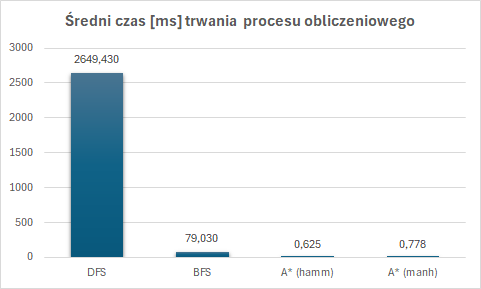
\includegraphics[width=\textwidth,height=\textheight,keepaspectratio]{average-time-with-dfs}
        \caption{Średni czas trwania procesu obliczeniowego dla odległości od rozwiązania równej 1-7.}
        \label{fig:1}
    \end{figure}

    \begin{figure}[!h]
        \centering
        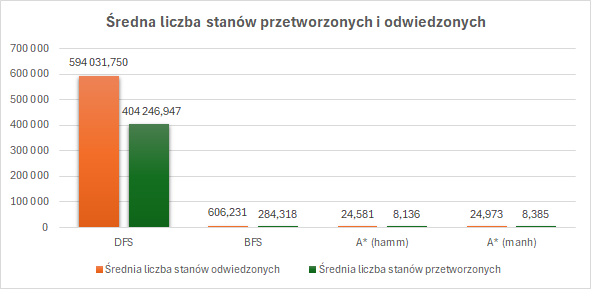
\includegraphics[width=\textwidth,height=\textheight,keepaspectratio]{average-count-of-visited-with-dfs}
        \caption{Średnia liczba stanów przetworzonych i odwiedzonych dla odległości od rozwiązania równej 1-7.}
        \label{fig:2}
    \end{figure}



    \begin{figure}
        \centering
        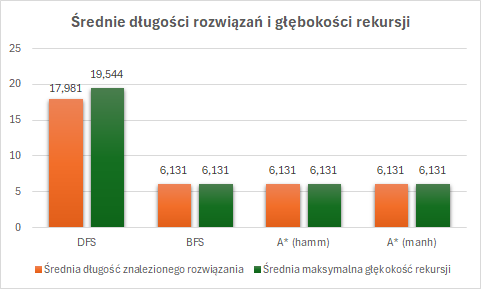
\includegraphics[width=\textwidth,height=\textheight,keepaspectratio]{average-solution-lenghts}
        \caption{Średnia długość rozwiązań i głębokość rekursji  dla odległości od rozwiązania 1-7. }
        \label{fig:3}
    \end{figure}

    \begin{figure}[!h]
        \centering
        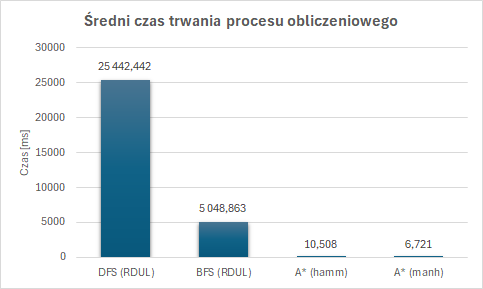
\includegraphics[width=\textwidth,height=\textheight,keepaspectratio]{average-time-for-big-grapth}
        \caption{Średni czas trwania procesu obliczeniowego dla odległości od rozwiązania równej 15.}
        \label{fig:6}
    \end{figure}
    \begin{figure}[!h]
        \centering
        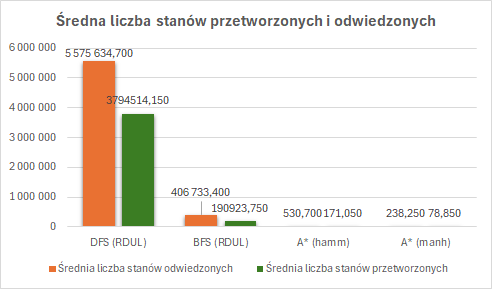
\includegraphics[width=\textwidth,height=\textheight,keepaspectratio]{average-count-of-visited-for-big-graph}
        \caption{Średnia liczba stanów przetworzonych i odwiedzonych dla odległości od rozwiązania równej 15.}
        \label{fig:7}
    \end{figure}
  }\label{sec:wyniki}
    \section{Dyskusja}
    {

        Na podstawie przeprowadzonych badań można wysunąć następujące wnioski:
         \begin{itemize}
         \setlength\itemsep{1em}
            \item {\textbf{Dla układów z głębokością rozwiązania 1-7}}
                \begin{itemize}

                    \item{Najgorsze efekty uzyskano przy pomocy metody DFS.
            Objawia się to znacznie dłuższym czasem szukania rozwiązania oraz odjandywaniem rozwiązań losowych a niekoniecznie najkrótszych.}

                    \item{ Metoda BFS zawsze znajduje najkrótsze rozwiazanie, jest to spowodowane sposobem działania metody, która sprawdza wszyskie mozliwe układy na zadanej głębokości przed sprawdzeniem kolejnej.}

                    \item{Metoda A* również zawsze odnajduje najkrótsze rozwiązanie, do tego metoda zdecydowanie najszybicej odnajdywała poprawne rozwiązanie.
            Różnicę pomiędzy wykorzystanymi heurystykami dla układów z głębokością 1-7 jest znikoma.}
                \end{itemize}
            \item {\textbf{Dla układów z głębokością rozwiązania 15}}
                 \begin{itemize}

                    \item { A* nadal jest najszybszą metodą spośród badanych, odnajdującą najkrótsze rozwiązanie.Dla tej głębokości różnice pomiędzy heurystykami stają się dużo bardziej widoczne, Manhattan jest zdecydowanie bardziej wydajny, osiągając nawet dwukrotnie lepsze wyniki niż Hamming.}

                    \item{Metoda DFS również wygenerowała poprawne wyniki.}

                    \item{Metoda BFS przez konieczność zapamiętywania wszyskich wężłów na danej głębokości.
            nie jest w stanie ukończyć rozwiązywania zadania (ograniczony rozmiar pamięci operacyjnej).}
                \end{itemize}
            \end{itemize}

      }\label{sec:dyskusja}

    \section{Wnioski}
    {
        \begin{itemize}
            \item A* okazał się najbardziej uniwersalną oraz optmalną metodą przeszukiwania grafów zarówno dla małych jak i duzych odległości układanek od układu wzorcowego. Początkowo znikome różnice pomiędzy heurystykami wzrastają wraz z głębokością rozwiązania układanki. Dla dużych głębokości Manhattan jest
            znacząco wydajniejszy.
            \item DFS również był w stanie odnaleźć rozwiązania dla każdego zadanego ułożenia układanki, jednak czas potrzebny na rozwiązanie był znaczie większy,
            w szczególności, w przypadku, gdy długość najkrótszego rozwiazania była znacznie mniejsza niż zadana głębokość poszukiwań.
            \item BFS dobrze poradził sobie z przeszukiwaniem układów o małej odległości od układu wzorcowego, jednak dla dużych odległości okazał się zupełnie niezdatny do użytku.
        \end{itemize}



    }\label{sec:wnioski}

    \begin{thebibliography}{0}
        \bibitem{l2short}
        \textsl{https://personal.math.ubc.ca/~cass/courses/m308-02b/projects/grant/fifteen.html}
    \end{thebibliography}


\end{document}